\chapter{MULTIPLY-ACCUMULATOR}
\label{chp:mac}
A high throughput SpMV implementation relies on designing a no-stall multiply accumulator (MAC). An inefficient engine will often stall when a matrix and its associated vector value arrives every or nearly every clock cycle. The long latency of floating point addition and row-column-row traversal makes this complicated.

\section{Related Work}
\label{sec:mac_related_work}
We looked at several multiply-accumulator designs before creating our own. We also use floating-point cores from Flopoco, so we are not starting from scratch. There are many different floating-point multiply-accumulators that solve different problems. Most accept one matrix element and one $x$ vector value at a time, however, we also discuss one that does not.
\subsection{Floating Point Adder and Multiplier (Flopoco)}
Most designs, including ours, use existing double-precision adder and multiplier cores for their multiply accumulator. We use Flopoco and use the features of these cores for analyzing other designs (See Table \ref{tbl:flopoco}) [\cite{prelim:dedinechin,prelim:banescu,prelim:dedinechin2}]. Flopoco uses a slightly different floating point format than the IEEE 754 standard. In addition to the floating-point adder and the floating-point multiplier we used 2 cores for converting to and from IEEE 754 format.

\begin{table}
    \caption{Flopoco Core Information}
    \label{tbl:flopoco}
    \begin{tabular}{|c|ccccc|}
        \hline
        IP Core & LUTs & Registers & DSPs & Frequency & \shortstack{Pipeline\\Stages} \\
        \hline
        \shortstack{Adder\\(FPAdder\_11\_52\_uid2)} & 1,190 & 1,136 & 0 & 298Mhz & 14 \\
        \hline
        \shortstack{Multiplier\\(FPMultiplier\_11\_52\_11\_52\_11\_52\_uid2)} & 1,067 & 1,061 & 7 & 314Mhz & 11 \\
        \hline
        \shortstack{IEEE 754 to Flopoco\\(InputIEEE\_11\_52)} & 67 & 68 & 0 & 280Mhz & 1 \\
        \hline
        \shortstack{Flopoco to IEEE 754\\(OutputIEEE\_11\_52)} & 65 & 67 & 0 & 260Mhz & 1 \\
        \hline
    \end{tabular}
\end{table}

\subsection{Binary Tree Accumulator}
Generally one multiplier multiplicand pair is sent per clock cycle to a multiply-accumulator, however one design streams multiple values at a time [\cite{prelim:sun2}]. Effectively, this MAC can be used to create a large processing element rather than many smaller ones. We have a slightly simplified version in \figurename~\ref{fig:tree_accumulator}. From a high level you can see this hardware computes dot-products. However, because the dot-products are of variable length the design is more complex.

\par This binary tree accumulator design uses an IPV (Input Pattern Vector) or bitmap to keep track of the rows. A `1' indicates the element is the last element in the row and a `0' otherwise. Our example MAC accepts 4 pairs of values per clock cycle. To explain this MAC let us use the example matrix from Equaiton~\ref{eqn:example}. The inputs in this case would be as follows:
\begin{enumerate}
    \item IPV=0010, data=($A_{11}\times x_1, A_{14}\times x_4, A_{17}\times x_7, A_{25}\times x_5$)
    \item IPV=1000, data=($A_{28}\times x_8, A_{32}\times x_2, A_{33}\times x_3, A_{36}\times x_6$)
    \item IPV=1010, data=($A_{37}\times x_7, A_{41}\times x_1, A_{45}\times x_5, A_{53}\times x_3$)
    \item IPV=0010, data=($A_{54}\times x_4, A_{57}\times x_7, A_{58}\times x_8, A_{62}\times x_2$)
    \item IPV=1000, data=($A_{65}\times x_5, A_{72}\times x_2, A_{73}\times x_3, A_{76}\times x_6$)
    \item IPV=1001, data=($A_{78}\times x_8, A_{83}\times x_3, A_{84}\times x_4, A_{86}\times x_6$)
\end{enumerate}
\begin{figure}
    \centering
    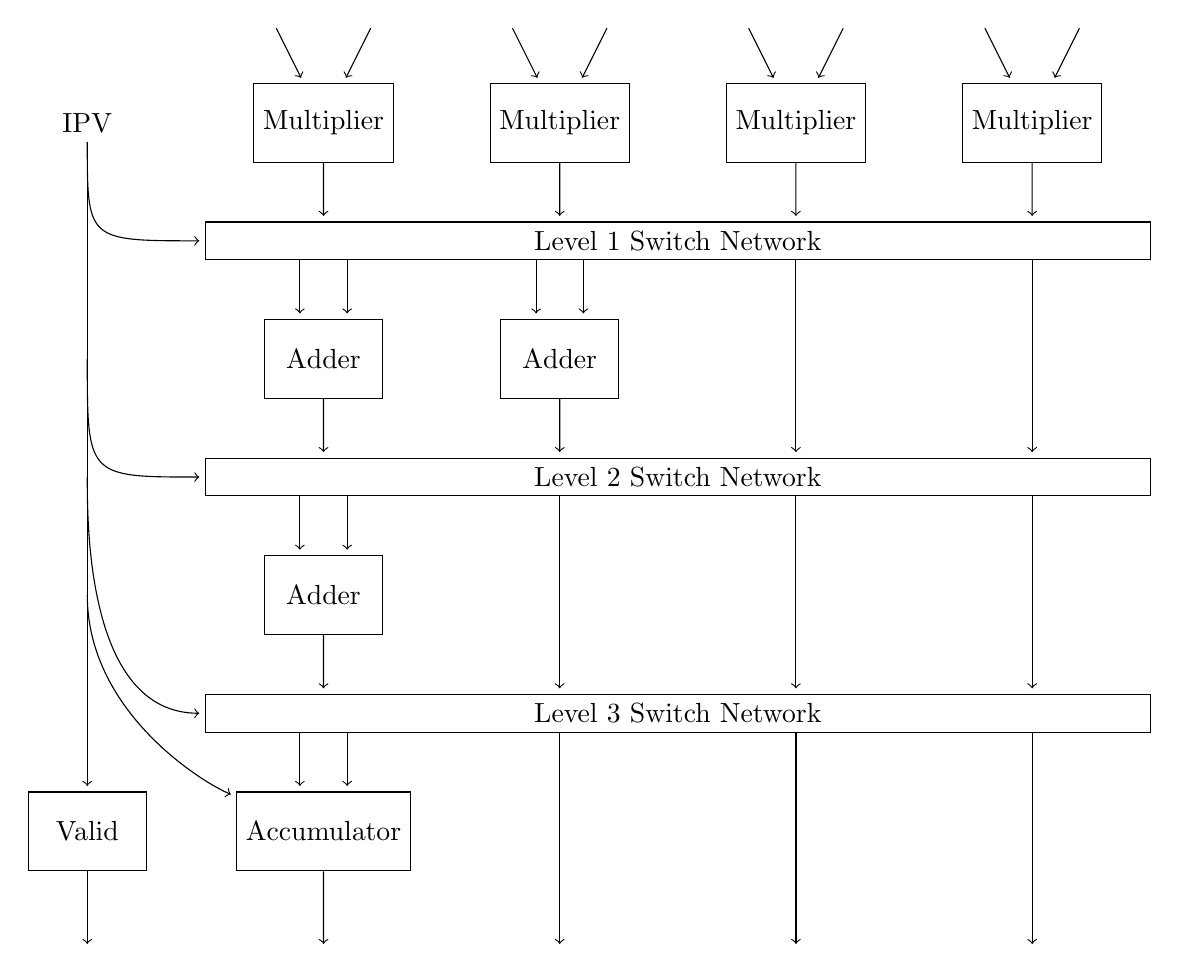
\begin{tikzpicture}[scale=3]
        \node(m0) at (1,0) [draw, minimum height=1cm]{Multiplier};
        \node(m1) at (2,0) [draw, minimum height=1cm]{Multiplier};
        \node(m2) at (3,0) [draw, minimum height=1cm]{Multiplier};
        \node(m3) at (4,0) [draw, minimum height=1cm]{Multiplier};

        \node(ipv) at (0,0) {IPV};

        \node(l1) at (2.5,-.5) [draw,minimum width=12cm]{Level 1 Switch Network};
        \node(l2) at (2.5,-1.5) [draw,minimum width=12cm]{Level 2 Switch Network};
        \node(l3) at (2.5,-2.5) [draw,minimum width=12cm]{Level 3 Switch Network};

        \node(a0) at (1,-1) [draw, minimum width=1.5cm, minimum height=1cm] {Adder};
        \node(a1) at (2,-1) [draw, minimum width=1.5cm, minimum height=1cm] {Adder};
        \node(a2) at (1,-2) [draw, minimum width=1.5cm, minimum height=1cm] {Adder};

        \node(acc) at (1,-3) [draw, minimum width=1.5cm, minimum height=1cm] {Accumulator};
        \node(valid) at (0, -3) [draw, minimum width=1.5cm, minimum height=1cm] {Valid};

        \draw[->,shorten >=2pt] (.8,.4) -- (m0);
        \draw[->,shorten >=2pt] (1.2,.4) -- (m0);
        \draw[->,shorten >=2pt] (1.8,.4) -- (m1);
        \draw[->,shorten >=2pt] (2.2,.4) -- (m1);
        \draw[->,shorten >=2pt] (2.8,.4) -- (m2);
        \draw[->,shorten >=2pt] (3.2,.4) -- (m2);
        \draw[->,shorten >=2pt] (3.8,.4) -- (m3);
        \draw[->,shorten >=2pt] (4.2,.4) -- (m3);

        \draw[->,shorten >=2pt] (m0) -- (l1.north -| m0);
        \draw[->,shorten >=2pt] (m1) -- (l1.north -| m1);
        \draw[->,shorten >=2pt] (m2) -- (l1.north -| m2);
        \draw[->,shorten >=2pt] (m3) -- (l1.north -| m3);

        \draw[->,shorten >=2pt](l1.south -| 1.1,0) -- (a0.north -| 1.1,0);
        \draw[->,shorten >=2pt](l1.south -| .9,0) -- (a0.north -| .9,0);

        \draw[->,shorten >=2pt](l1.south -| 2.1,0) -- (a1.north -| 2.1,0);
        \draw[->,shorten >=2pt](l1.south -| 1.9,0) -- (a1.north -| 1.9,0);

        \draw[->,shorten >=2pt](l2.south -| 1.1,0) -- (a2.north -| 1.1,0);
        \draw[->,shorten >=2pt](l2.south -| 0.9,0) -- (a2.north -| 0.9,0);

        \draw[->,shorten >=2pt](l3.south -| 1.1,0) -- (acc.north -| 1.1,0);
        \draw[->,shorten >=2pt](l3.south -| 0.9,0) -- (acc.north -| 0.9,0);

        \draw[->,shorten >=2pt](a0) -- (l2.north -| a0);
        \draw[->,shorten >=2pt](a1) -- (l2.north -| a1);
        \draw[->,shorten >=2pt](a2) -- (l3.north -| a2);

        \draw[->,shorten >=2pt](l1.south -| m2) -- (l2.north -| m2);
        \draw[->,shorten >=2pt](l1.south -| m3) -- (l2.north -| m3);

        \draw[->,shorten >=2pt](l2.south -| m1) -- (l3.north -| m1);
        \draw[->,shorten >=2pt](l2.south -| m2) -- (l3.north -| m2);
        \draw[->,shorten >=2pt](l2.south -| m3) -- (l3.north -| m3);

        \draw[->,shorten >=2pt](valid) -- (valid |- 0,-3.5);
        \draw[->,shorten >=2pt](acc) -- (acc |- 0,-3.5);
        \draw[->,shorten >=2pt](l3.south -| 2,0) -- (2,0 |- 0,-3.5);
        \draw[->,shorten >=2pt](l3.south -| 3,0) -- (3,0 |- 0,-3.5);
        \draw[->,shorten >=2pt](l3.south -| 4,0) -- (4,0 |- 0,-3.5);

        \draw[->,shorten >=2pt](ipv) -- (valid);
        \draw[->,shorten >=2pt](ipv) .. controls +(0,-.5) and +(-.5,0) .. (l1.west);
        \draw[->,shorten >=2pt](0,-1) .. controls +(0,-.5) and +(-.5,0) .. (l2.west);
        \draw[->,shorten >=2pt](0,-1.5) .. controls +(0,-.2) and +(-.5,0) .. (l3.west);
        \draw[->,shorten >=2pt](0,-2) .. controls +(0,-.5) and +(-.5,.2) .. (acc);

    \end{tikzpicture}
    \caption{Binary Tree Accumulator}
    \label{fig:tree_accumulator}
\end{figure}

\begin{table}
    \caption{Operation of the binary tree accumulator based on the IPV}
    \label{tbl:ipv}
    \begin{tabular}{|c|c|c|c|c|}
        \hline
        IPV & 0010 & 1000 & 1010 & 1001 \\ 
        \hline
        \shortstack{Level 1\\Switch\\Network} &
        \shortstack{$\textrm{IN}_0 \rightarrow \textrm{OUT}_0$\\
        $\textrm{IN}_1 \rightarrow \textrm{OUT}_1$\\
    $\textrm{IN}_2 \rightarrow \textrm{OUT}_2$\\
$\textrm{IN}_3 \rightarrow \textrm{OUT}_4$\\
$0 \rightarrow \textrm{OUT}_3$\\
$0 \rightarrow \textrm{OUT}_5$} &
        \shortstack{$\textrm{IN}_0 \rightarrow \textrm{OUT}_0$\\
        $\textrm{IN}_1 \rightarrow \textrm{OUT}_2$\\
        $\textrm{IN}_2 \rightarrow \textrm{OUT}_3$\\
    $\textrm{IN}_3 \rightarrow \textrm{OUT}_4$\\
$0 \rightarrow \textrm{OUT}_1$\\
$0 \rightarrow \textrm{OUT}_5$} &
\shortstack{$\textrm{IN}_0 \rightarrow \textrm{OUT}_0$\\
$\textrm{IN}_1 \rightarrow \textrm{OUT}_2$\\
$\textrm{IN}_2 \rightarrow \textrm{OUT}_3$\\
$\textrm{IN}_3 \rightarrow \textrm{OUT}_4$\\
$0 \rightarrow \textrm{OUT}_3$\\
$0 \rightarrow \textrm{OUT}_5$} &
\shortstack{$\textrm{IN}_0 \rightarrow \textrm{OUT}_0$\\
$\textrm{IN}_1 \rightarrow \textrm{OUT}_2$\\
$\textrm{IN}_2 \rightarrow \textrm{OUT}_3$\\
$\textrm{IN}_3 \rightarrow \textrm{OUT}_4$\\
$0 \rightarrow \textrm{OUT}_0$\\
$0 \rightarrow \textrm{OUT}_5$}\\
        \hline
        \shortstack{Level 2\\Switch\\Network} &
\shortstack{$\textrm{IN}_0 \rightarrow \textrm{OUT}_0$\\
$\textrm{IN}_1 \rightarrow \textrm{OUT}_1$\\
$\textrm{IN}_2 \rightarrow \textrm{OUT}_2$\\
$\textrm{IN}_3 \rightarrow \textrm{OUT}_3$\\
$0 \rightarrow \textrm{OUT}_4$} &
\shortstack{$\textrm{IN}_0 \rightarrow \textrm{OUT}_2$\\
$\textrm{IN}_1 \rightarrow \textrm{OUT}_0$\\
$\textrm{IN}_2 \rightarrow \textrm{OUT}_1$\\
$\textrm{IN}_3 \rightarrow \textrm{OUT}_3$\\
$0 \rightarrow \textrm{OUT}_4$} &
\shortstack{$\textrm{IN}_0 \rightarrow \textrm{OUT}_0$\\
$\textrm{IN}_1 \rightarrow \textrm{OUT}_2$\\
$\textrm{IN}_2 \rightarrow \textrm{OUT}_3$\\
$\textrm{IN}_3 \rightarrow \textrm{OUT}_4$\\
$0 \rightarrow \textrm{OUT}_1$} &
\shortstack{$\textrm{IN}_0 \rightarrow \textrm{OUT}_2$\\
$\textrm{IN}_1 \rightarrow \textrm{OUT}_0$\\
$\textrm{IN}_2 \rightarrow \textrm{OUT}_1$\\
$\textrm{IN}_3 \rightarrow \textrm{OUT}_3$\\
$0 \rightarrow \textrm{OUT}_4$}\\

        \hline
        \shortstack{Level 3\\Switch\\Network} &
            \shortstack{$\textrm{IN}_0 \rightarrow \textrm{OUT}_1$\\
$\textrm{IN}_1 \rightarrow \textrm{OUT}_0$\\
$\textrm{IN}_2 \rightarrow \textrm{OUT}_2$\\
$\textrm{IN}_3 \rightarrow \textrm{OUT}_3$\\
$0 \rightarrow \textrm{OUT}_4$} &
\shortstack{$\textrm{IN}_0 \rightarrow \textrm{OUT}_0$\\
$\textrm{IN}_1 \rightarrow \textrm{OUT}_1$\\
$\textrm{IN}_2 \rightarrow \textrm{OUT}_2$\\
$\textrm{IN}_3 \rightarrow \textrm{OUT}_3$\\
$0 \rightarrow \textrm{OUT}_4$} &
\shortstack{$\textrm{IN}_0 \rightarrow \textrm{OUT}_1$\\
$\textrm{IN}_1 \rightarrow \textrm{OUT}_2$\\
$\textrm{IN}_2 \rightarrow \textrm{OUT}_0$\\
$\textrm{IN}_3 \rightarrow \textrm{OUT}_3$\\
$0 \rightarrow \textrm{OUT}_4$} &
\shortstack{$\textrm{IN}_0 \rightarrow \textrm{OUT}_2$\\
$\textrm{IN}_1 \rightarrow \textrm{OUT}_1$\\
$\textrm{IN}_2 \rightarrow \textrm{OUT}_0$\\
$\textrm{IN}_3 \rightarrow \textrm{OUT}_3$\\
$0 \rightarrow \textrm{OUT}_4$}\\

        \hline
        valid & 1000 & 1000 & 1100 & 1100 \\ 
        \hline
    \end{tabular}
\end{table}
You may notice that this computation does the additions out of order. For an example of out of order addition, when computing $1+2+3+4$ the MAC does $(1+2)+(3+4)$. This removes the data dependency of adding $1$ and $2$ before processing $3$. CPUs and GPUs (in general) compute floating point addition in order (eg. $\left((1+2)+3\right)+4$). This means results may differ slightly, because changing the order of floating point addition can change the result [\cite{prelim:goldberg}].

%\subsection{Log Sum Accumulator}
\begin{figure}
    \centering
    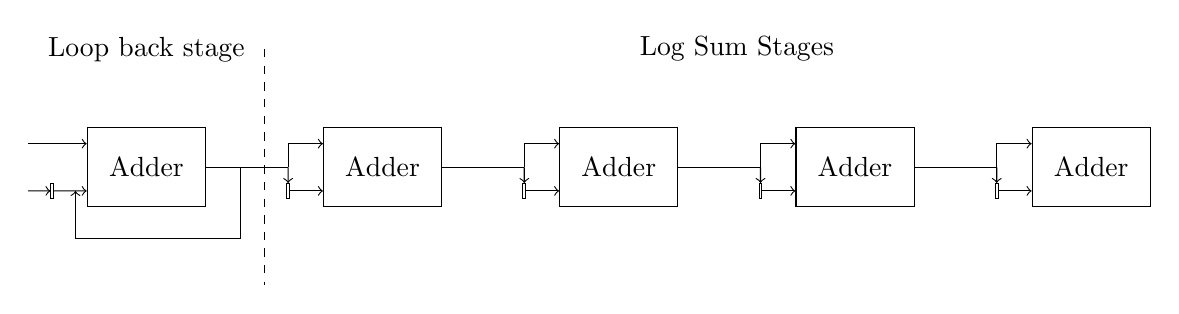
\begin{tikzpicture}[scale=3]
        \node(a) at (0,0) [draw,minimum width=1.5cm, minimum height=1cm]{Adder};
        \node(b) at (1,0) [draw,minimum width=1.5cm, minimum height=1cm]{Adder};
        \node(c) at (2,0) [draw,minimum width=1.5cm, minimum height=1cm]{Adder};
        \node(d) at (3,0) [draw,minimum width=1.5cm, minimum height=1cm]{Adder};
        \node(e) at (4,0) [draw,minimum width=1.5cm, minimum height=1cm]{Adder};
        \draw[->] (-.5,.1) -- (a.west |- -.5,.1);
        \node(r0) at (-.4,-.1) [draw, inner sep=0pt, outer sep=0pt,minimum height=.2cm] {};
        \draw[->] (-.5,-.1) -- (r0);
        \draw[->] (r0) -- (a.west |- -.5,-.1);
        \draw[] (a.east) -- (.6,0);
        \draw[->] (.4,0) -- (.4,-.3) -- (-.3,-.3) -- (-.3,-.1);
        \draw[->] (.6,0) -- (.6,.1) -- (b.west |- .6,.1);
        \node(r1) at (0.6,-.1) [draw, inner sep=0pt, outer sep=0pt,minimum height=.2cm] {};
        \node(r2) at (1.6,-.1) [draw, inner sep=0pt, outer sep=0pt,minimum height=.2cm] {};
        \node(r3) at (2.6,-.1) [draw, inner sep=0pt, outer sep=0pt,minimum height=.2cm] {};
        \node(r4) at (3.6,-.1) [draw, inner sep=0pt, outer sep=0pt,minimum height=.2cm] {};
        \draw[->] (.6,0) -- (r1);
        \draw[->] (r1) -- (b.west |- r1);

        \draw[] (b) -- (1.6,0);
        \draw[->] (1.6,0) -- (1.6,.1) -- (c.west |- .6,.1);
        \draw[->] (1.6,0) -- (r2);
        \draw[->] (r2) -- (c.west |- r2);

        \draw[] (c) -- (2.6,0);
        \draw[->] (2.6,0) -- (2.6,.1) -- (d.west |- .6,.1);
        \draw[->] (2.6,0) -- (r3);
        \draw[->] (r3) -- (d.west |- r3);

        \draw[] (d) -- (3.6,0);
        \draw[->] (3.6,0) -- (3.6,.1) -- (e.west |- .6,.1);
        \draw[->] (3.6,0) -- (r4);
        \draw[->] (r4) -- (e.west |- r4);

        \draw[dashed] (.5,.5) -- (.5,-.5);
        \node at (0,.5){Loop back stage};
        \node at (2.5,.5){Log Sum Stages};
    \end{tikzpicture}
    \caption{Log Sum Accumulator}
\end{figure}

\subsection{Single Adder Accumulator}
A multiply-accumulator with one multiplier should only need one adder to do all the accumulation. You may have noticed that the adders get progressively underutilized in the log-sum accumulator. The difficulty is how to create an algorithm to achieve this. It is clear that buffering has to occur to achieve this. If the output needs to be in order than the buffering needs to be at least $O(a\textrm{log}(a))$ to accomadate the case where one row has several valuse and fills the adder pipeline and the following rows have only 1 value. If the output can be out of order (meaning the output of the short rows that get accumulated quickly can go to the output before the long rows before it) than it seems like $O(a)$ is the lower limit of the required buffering.

Other work has achieved accumulators with $O(1)$ adders. \cite{prelim:zhuo} came up with 2 accumulators that use 2 adders and 1 that uses a single adder. However, the single adder solution had restrictions. In addition to only allowing row-major traversal it had a maximum row length of $a$ (the depth of the adder pipeline). This design also required $O(a^2)$ buffer space. The accumulator has two buffers. While one buffer is having it's values accumulated the other is recieving new values. The adder takes in two values from the buffer in the accumulation state and then jumps $a$ addresses to add two other values that belong to a different row. Table~\ref{tbl:single_adder} shows the schedualing of accumulating the products from the example in Equation~\ref{eqn:example}. For simplification we set $\alpha = 4$ instead of $\alpha = 14$.

Some may notice a hazard occurs if two value in the fourth column of the buffer belong to the same row of the matrix. This is what prevents this accumulator from being able to accumulate rows greater than $\alpha$. To accomadate this case the accumulator could have an additional adder or stall the accumulator to allow time for accumulating the long rows.

\begin{sidewaystable}
    \centering
    \caption{A single adder accumulator}
    \label{tbl:single_adder}
    \begin{tabular}{|c||c|c|c|c||c||c|c|c|c|}
        \hline
        Cycle & \multicolumn{4}{c||}{First buffer} & Adder & \multicolumn{4}{c|}{Second buffer} \\
        \hline
        \hline
        \multirow{4}{*}{1-4} & $A_{11}x_1$ & $A_{14}x_4$ & $A_{17}x_7$ & $A_{25}x_5$ & & & & & \\
        \cline{2-10}
        & $A_{28}x_8$ & $A_{32}x_2$ & $A_{33}x_3$ & $A_{36}x_6$ & & & & & \\
        \cline{2-10}
        & $A_{37}x_7$ & $A_{41}x_1$ & $A_{45}x_5$ & $A_{53}x_3$ & & & & & \\
        \cline{2-10}
        & $A_{54}x_4$ & $A_{57}x_7$ & $A_{58}x_8$ & $A_{62}x_2$ & & & & & \\
        \hline
        \hline
        \multirow{4}{*}{5-8} & & & $A_{17}x_7$ & $A_{25}x_5$ & $A_{11}x_1 + A_{14}x_4$ & $A_{65}x_5$ & $A_{72}x_2$ & $A_{73}x_3$ & $A_{76}x_6$ \\
        \cline{2-10}
        & $A_{28}x_8$ & $A_{32}x_2$ & $A_{33}x_3$ & $A_{36}x_6$ & & & & & \\
        \cline{2-10}
        & $A_{37}x_7$ & $A_{41}x_1$ & $A_{45}x_5$ & $A_{53}x_3$ & & & & & \\
        \cline{2-10}
        & & & $A_{58}x_8$ & $A_{62}x_2$ & $A_{54}x_4 + A_{57}x_7$ & & & & \\
        \hline
        \hline
        \multirow{4}{*}{9-12} & & & & $A_{25}x_5$ & $\left(A_{11}x_1 + A_{14}x_4\right) + A_{17}x_7$ & $A_{65}x_5$ & $A_{72}x_2$ & $A_{73}x_3$ & $A_{76}x_6$ \\
        \cline{2-10}
        & $A_{28}x_8$ & & & $A_{36}x_6$ & $A_{32}x_2 + A_{33}x_3$ & $A_{78}x_8$ & $A_{83}x_3$ & $A_{84}x_4$ & $A_{85}x_5$\\
        \cline{2-10}
        & $A_{37}x_7$ & & & $A_{53}x_3$ & $A_{41}x_1 + A_{45}x_5$ & & & & \\
        \cline{2-10}
        & & & & $A_{62}x_2$ & $\left(A_{54}x_4 + A_{57}x_7\right) + A_{58}x_8$ & & & & \\
        \hline
        \hline
        \multirow{4}{*}{13-16} & & & & $A_{25}x_5$ & & $A_{65}x_5$ & $A_{72}x_2$ & $A_{73}x_3$ & $A_{76}x_6$ \\
        \cline{2-10}
        & $A_{28}x_8$ & & & & $\left(A_{32}x_2 + A_{33}x_3\right) + A_{36}x_6$ & $A_{78}x_8$ & $A_{83}x_3$ & $A_{84}x_4$ & $A_{85}x_5$\\
        \cline{2-10}
        & $A_{37}x_7$ & & & $A_{53}x_3$ & & $A_{86}x_6$ & & & \\
        \cline{2-10}
        & $A_{54}x_4 + A_{57}x_7 + A_{58}x_8$ & & & & $A_{62}x_2$ & & & & \\
        \hline
        \hline
        \multirow{4}{*}{17-20} & & & & & & $A_{65}x_5$ & $A_{72}x_2$ & $A_{73}x_3$ & $A_{76}x_6$ \\
        \cline{2-10}
        & & & & & $A_{25}x_5 + A_{28}x_8$ & $A_{78}x_8$ & $A_{83}x_3$ & $A_{84}x_4$ & $A_{85}x_5$\\
        \cline{2-10}
        & & & & & $\left(A_{32}x_2 + A_{33}x_3 + A_{36}x_6\right) + A_{37}x_7$ & $A_{86}x_6$ & & & \\
        \cline{2-10}
        & & & & & $A_{53}x_3 + \left(A_{54}x_4 + A_{57}x_7 + A_{58}x_8\right)$ & & & & \\
        \hline


    \end{tabular}
\end{sidewaystable}

\subsection{Using a single cycle Accumulation loop}
Another solution to this problem is to accumulate in one clock cycle. This is the approach in [\cite{prelim:bachir}]. The idea is to split the accumulation into 3 phases: The extend mantissa and reduce exponent phase, the accumulation loop phase, and the normalize phase. In the first phase the floating point format is converted into a 5-bit exponent and a 52+64=116-bit 2s complement mantissa. In the second phase the incomming value is added to the stored value. In the third phase, the stored value is converted back into IEEE-754 format.

The accumulation phase is more complex than a simple 2s complement adder, because there is an exponent. The difference in the exponents determines what operation the accumulator does. If the incoming exponent $e_i$ is more than 2 greater than the stored exponent $e_s$ than the stored value is thrown out because it is too small and the incomming value replaces the stored value. The other cases are in Table~\ref{tbl:accumulator_ops}.

\begin{table}
    \caption{Based on the difference of the incomming exponent $e_i$ and the stored exponent $e_s$ the accumulator does a different operation to add the two values together}
    \label{tbl:accumulator_ops}
    \begin{tabular}{|c|c|}
        \hline
        $e_s - e_i$ & $e_i\Leftarrow$ \\
        \hline
    \end{tabular}
\end{table}

As you may guess this is still a lot of logic for one clock cycle and as a result this limit the maximum frequency.

\section{Multiply-accumulator with an Intermediator}
\label{sec:intermediator}
The problem with all these designs is that they require row-major traversal. This handicap makes these MACs unusable for our purposes. The requirements fo our MAC is as follows:
\begin{enumerate}
    \item Within a 512 row section the MAC can recieve elements in any order.
    \item The MAC must recieve all the elements in one 512 row section before proceeding to the next 512 row section.
    \item Each row must have at least one element.
    \item The MAC can stall, but not stall often enough to significantly effect throughput.

\end{enumerate}
To achieve this we created a MAC that uses one multilier and one adder and one Intermediator block (see \figurename~\ref{fig:mac}). This Intermediator stores up to one intermediate $y$ value for each row in a dual port RAM. This RAM is central to the design of the Intermediator.

\par In $R^3$ [\cite{prelim:townsend}] we introduced the Intermediator but it was only capable of storing 32 intermediate $y$ vector values (see figure \ref{fig:mac}). In this design, we expand this to 1024 (the minimum depth of one dual port RAM block in most Xilinx, Altera and Lattice FPGAs). Both Intermediator designs allow the matrix to be traversed in a loosely row major traversal and the MAC still works correctly. The step from 32 to 1024 intermediate values allows more freedom in the traversal. Earlier in Chapter \ref{chp:traversal} we discussed traversals that abide by this rule and allow for easy reuse of $x$ vector values.


\begin{figure}
    \centering
\begin{tikzpicture}[scale=1]
\clip (-5,-2.5) rectangle (5,2.5);
\node at (0,0) [draw, rectangle, minimum height=4cm, minimum width=8cm, label={[label distance=-.6cm,xshift=-2cm]90:Multiply-Accumulator}](acc){};
\node at (acc) [draw, rectangle, xshift=3cm, yshift=0cm, minimum height=1cm, minimum width=2cm](add){Adder};
\node at (acc) [draw, rectangle, xshift=.3cm, yshift=0cm, minimum height=1cm, minimum width=0](int){\shortstack{Intermediator}};
\node at (acc) [draw, rectangle, xshift=-3cm, yshift=0cm, minimum height=1cm, minimum width=2cm](mult){\shortstack{Multiplier}};

\path [draw, thick, >=stealth',->] (-5,.3) --node[ fill=white, inner sep=1pt]{val} (-4,.3) ;
\path [draw, thick, >=stealth',->] (-5,0) --node[ fill=white, inner sep=1pt]{val} (-4,0) ;
\path [draw, thick, >=stealth',->] (-5,-.3) --node[ fill=white, inner sep=1pt]{row} (-4,-.3);

\path [draw, thick, >=stealth',->] (-2,0) --node[ fill=white, inner sep=1pt]{val} (-1,0);
\path [draw, thick, >=stealth',->] (-2,-.3) --node[ fill=white, inner sep=1pt]{row} (-1,-.3) ;

\path [draw, thick, >=stealth',->] (.4,.5)  arc(160:20:1.2);
\node at (1.5,1.2)[fill=white, inner sep=1pt]{row};

\path [draw, thick, >=stealth',->] (.1,.5)  arc(163:17:1.5);
\node at (1.5,1.5)[fill=white, inner sep=1pt]{val};

\path [draw, thick, >=stealth',->] (-.2,.5)  arc(166:14:1.8);
\node at (1.5,1.8)[fill=white, inner sep=1pt]{val};

\path [draw, thick, >=stealth',->] (2.6,-.5)  arc(-20:-160:1.2);
\node at (1.5,-1.2)[fill=white, inner sep=1pt]{row};

\path [draw, thick, >=stealth',->] (2.9,-.5)  arc(-17:-163:1.5);
\node at (1.5,-1.5)[fill=white, inner sep=1pt]{val};

\path [draw, thick, >=stealth',->] (-.5,-.5) --node[sloped, fill=white, inner sep=1pt]{val} (-.5,-2.5);
\end{tikzpicture} %

\caption[Multiply-accumulator]{The no-stall multiply-accumulator block handles multiple intermediate values at a time. This allows multiple intermediate values in the adder pipeline.}
\label{fig:mac}
\end{figure}
\subsection{Memory and States}
The RAM block in the Intermediator has a depth of 1024. Each slot in memory has 2 types of states. First, each slot is either occupied or vacant. Second, each slot in either the red (active), yellow (fading), green (accumulated), or white (blank) states.

The memory is split in 2, an upper and lower section. Once the accumulation starts, one of these sections will be in the red active state. Once the incoming values move to the next 512 row section of the matrix this section transitions to the yellow fading state, and the new section of the memory is now in the red active state. Recall our traversal rule is that each 512 rows must be traversed before proceeding to the next 512 rows. The yellow fading state exists because values are still being accumulated in the previously active memory. The memory will always be accumulated within 80 clock cycles. At that point the faded state transitions to the green state and ready to be stored. Once the values have been sent out to be stored the memory transitions to the white blank state.

\subsection{Operations}
The Intermediator (Figure \ref{intermediatorEx}) takes in two values, one from the multiplier's result and one from the adder's result and outputs a pair of values to be added together. The dual-port RAM block (the middle block in Figure \ref{intermediatorEx}) stores intermediate values until an element in the same row appears. \par

Ideally the Intermediator receives a value from the multiplier and one value from the adder every clock cycle. These values often belong to different rows. The Intermediator also outputs one pair of values belonging to the same row to the adder every clock cycle.

\par So the Intermediator plays a game where it receives 2 values belonging to different rows and sends 2 values belonging to the same row.

\par Many cases occur when accumulating values in multiple rows and the Intermediator handles each case properly:
\\\indent Case 1: (Figure \ref{cycle7}) The trivial case, no valid input arrives. If the ``to result" block has values, it outputs a pair of values to the adder. An overflow FIFO (explained in case 6) outputs a value if it has values.
\\\indent Case 2: (Figure \ref{cycle4}) Only one value arrives and the row corresponds to a vacant cell. The value goes into the vacant cell. If the ``to result" window has values, it outputs a result, and if the overflow FIFO has values it outputs a set to the adder.
\\\indent Case 3: (Figure \ref{cycle1}) Similar to case 2 except with an occupied cell. It retrieves the value in the Intermediator cell and goes to the adder with the input value. The state of the cell gets updated to vacant.
\\\indent Case 4: (Figure \ref{cycle2}, \ref{cycle8}) Both values have row indexes that correspond to vacant cells in the RAM block. Both values get stored in the RAM block and both cells switch to occupied. If the overflow FIFO has values it sends one set of values to the output. 
\\\indent Case 5: (Figure \ref{cycle6}) One value has a row index corresponding to a vacant cell, and the other to an occupied cell. The first value goes in the vacant cell and the value in the occupied cell goes to the adder with the second value. 
\\\indent Case 6: (Figure \ref{cycle3}) Both values have row indexes that correspond to occupied cells in the RAM. One input value and its corresponding Intermediator cell's value go to the output. The output can only handle one output pair at a time, so the other input value and its corresponding Intermediator cell's value go to the overflow FIFO.
\\\indent Case 7: (Figure \ref{cycle5}) The values have identical row indices. In this case, the values go through the pipeline and do not touch the Intermediator cells. They simply pass through to the adder.\\
%
To help explain, consider a simpler case where the depth of the intermediator is 8 instead of 1024. Figure \ref{intermediatorEx} shows 8 clock cycles of operation. At every clock cycle up to 2 valid input values with corresponding row indexes arrive. For simplicity, we do not show the values being calculated in the figure.
\begin{figure*}
\begin{multicols}{3}
\begin{subfigure}{\linewidth}
\begin{tikzpicture}
\node (a) {Input};
\node (b)[below=of a] {Result};
\node (c)[right=of a,xshift=-.6cm,yshift=.2cm] {RAM};
\draw (c) +(-.5,0.2) rectangle ++(.5,-2.2);
\node (d)[xshift=-.7cm,yshift=-.5cm,right=of c, draw, minimum width=1.5cm, minimum height=.5cm, label=above:FIFO]{};
\node (e1) at ([xshift=-.6cm]d) [draw, rectangle, minimum height=.5cm, minimum width=.3cm,pattern=north east lines]{};
\node (e)[below=of d, yshift=.3cm]{Adder};
%\node (f) at ([yshift=-2cm]c) [draw,minimum width=1.5cm]{};
%\coordinate (s16) at ($ (c) - (.5,0) $);
%\draw (s16) rectangle ++(.5,.5);
\foreach [count=\i] \y in {-1.85,-1.6,...,-.1}{
	\node (n\i) at ([xshift=-0cm,yshift=-.2cm+\y cm]c) [minimum height=.25cm, minimum width=1cm]{};
}
%\node (active) at ([xshift=.7cm,yshift=0cm]n5) [draw,fill=red!30,rectangle,minimum width=1cm,minimum height=.25cm]{};
\draw[pattern=north east lines,preaction={fill,red}] ([xshift=-.5cm,yshift=-.125cm]n5) rectangle ([xshift=.5cm,yshift=.125cm]n6);
\draw[preaction={fill,red}] ([xshift=-.5cm,yshift=-.125cm]n7) rectangle ([xshift=.5cm,yshift=.125cm]n8);
\draw[pattern=north east lines,preaction={fill,green}] ([xshift=-.5cm,yshift=-.125cm]n1) rectangle ([xshift=.5cm,yshift=.125cm]n4);
%\draw[pattern=north east lines,preaction={fill,green}] ([xshift=-.5cm,yshift=-.125cm]n2) rectangle ([xshift=.5cm,yshift=.125cm]n2);
\foreach [count=\i] \y in {-1.85,-1.6,...,-.1}{
    \FPeval{\n}{round(\i-1:0)}
	\node (m\i) at ([xshift=-0.7cm,yshift=-.2cm+\y cm]c) []{\scriptsize \n};
}

\path [draw, thick, >=stealth',->](a) to [bend right=20] (e);

\path [draw, thick, >=stealth',->](n1.west) to [bend right=0] (b);
\draw [->,thick, >=stealth'] (n6.east) to [bend left=10] (e);
%\tikzstyle{line} = [draw, thick, -latex' ,shorten >=2pt];
\end{tikzpicture}
\caption{First clock cycle, 1 pair of values get sent to the adder.}
\label{cycle1}
\end{subfigure}

\begin{subfigure}{\linewidth}
\begin{tikzpicture}
\node (a) {Input};
\node (b)[below=of a] {Result};
\node (c)[right=of a,xshift=-.6cm,yshift=.2cm] {RAM};
\draw (c) +(-.5,0.2) rectangle ++(.5,-2.2);
\node (d)[xshift=-.7cm,yshift=-.5cm,right=of c, draw, minimum width=1.5cm, minimum height=.5cm, label=above:FIFO]{};
\node (e1) at ([xshift=-.6cm]d) [draw, rectangle, minimum height=.5cm, minimum width=.3cm,pattern=north east lines]{};
\node (e)[below=of d, yshift=.3cm]{Adder};
%\node (f) at ([yshift=-2cm]c) [draw,minimum width=1.5cm]{};
%\coordinate (s16) at ($ (c) - (.5,0) $);
%\draw (s16) rectangle ++(.5,.5);
\foreach [count=\i] \y in {-1.85,-1.6,...,-.1}{
	\node (n\i) at ([xshift=-0cm,yshift=-.2cm+\y cm]c) [minimum height=.25cm, minimum width=1cm]{};
}
%\node (active) at ([xshift=.7cm,yshift=0cm]n5) [draw,fill=red!30,rectangle,minimum width=1cm,minimum height=.25cm]{};
\draw[fill=red] ([xshift=-.5cm,yshift=-.125cm]n5) rectangle ([xshift=.5cm,yshift=.125cm]n8);
\draw[pattern=north east lines] ([xshift=-.5cm,yshift=-.125cm]n5) rectangle ([xshift=.5cm,yshift=.125cm]n5);
\draw[pattern=north east lines,preaction={fill,green}] ([xshift=-.5cm,yshift=-.125cm]n2) rectangle ([xshift=.5cm,yshift=.125cm]n4);
\foreach [count=\i] \y in {-1.85,-1.6,...,-.1}{
    \FPeval{\n}{round(\i-1:0)}
	\node (m\i) at ([xshift=-0.7cm,yshift=-.2cm+\y cm]c) []{\scriptsize \n};
}

\path [draw, thick, >=stealth',->](a) to [bend right=20] (n6.west);
\path [draw, thick, >=stealth',->](a) to [bend right=10] (n7.west);
%\edge [draw, thick, ->, bend right] (e2.south) -- (e);
\draw [->,thick, >=stealth'] (e1) to [bend right=10] (e);
%\tikzstyle{line} = [draw, thick, -latex' ,shorten >=2pt];
\end{tikzpicture}
\caption{Second clock cycle, 2 values gets stored in the RAM.}
\label{cycle2}
\end{subfigure}

\begin{subfigure}{\linewidth}
\centering
\begin{tikzpicture}
\node (a) {Input};
\node (b)[below=of a] {Result};
\node (c)[right=of a,xshift=-.6cm,yshift=.2cm] {RAM};
\draw (c) +(-.5,0.2) rectangle ++(.5,-2.2);
\node (d)[xshift=-.7cm,yshift=-.5cm,right=of c, draw, minimum width=1.5cm, minimum height=.5cm, label=above:FIFO]{};
\node (e)[below=of d, yshift=.3cm]{Adder};
%\node (f) at ([yshift=-2cm]c) [draw,minimum width=1.5cm]{};
%\coordinate (s16) at ($ (c) - (.5,0) $);
%\draw (s16) rectangle ++(.5,.5);
\foreach [count=\i] \y in {-1.85,-1.6,...,-.1}{
	\node (n\i) at ([xshift=-0cm,yshift=-.2cm+\y cm]c) [minimum height=.25cm, minimum width=1cm]{};
}
%\node (active) at ([xshift=.7cm,yshift=0cm]n5) [draw,fill=red!30,rectangle,minimum width=1cm,minimum height=.25cm]{};
\draw[fill=red] ([xshift=-.5cm,yshift=-.125cm]n5) rectangle ([xshift=.5cm,yshift=.125cm]n8);
\draw[pattern=north east lines] ([xshift=-.5cm,yshift=-.125cm]n5) rectangle ([xshift=.5cm,yshift=.125cm]n7);
\draw[pattern=north east lines,preaction={fill,green}] ([xshift=-.5cm,yshift=-.125cm]n2) rectangle ([xshift=.5cm,yshift=.125cm]n4);
\foreach [count=\i] \y in {-1.85,-1.6,...,-.1}{
    \FPeval{\n}{round(\i-1:0)}
	\node (m\i) at ([xshift=-0.7cm,yshift=-.2cm+\y cm]c) []{\scriptsize \n};
}

\path [draw, thick, >=stealth',->](a) to [bend left=10] (d);
\path [draw, thick, >=stealth',->](n7.east) to [bend left=1] (d);
\path [draw, thick, >=stealth',->](a) to [bend right=0] (e);
\path [draw, thick, >=stealth',->](n6.east) to [bend left=30](e);
\end{tikzpicture}
\caption{Third clock cycle, the 2 inputs correspond to occupied cells in the RAM block.}
\label{cycle3}
\end{subfigure}

\end{multicols}
%
\begin{multicols}{3}
\begin{subfigure}{\linewidth}
\begin{tikzpicture}
\node (a) {Input};
\node (b)[below=of a] {Result};
\node (c)[right=of a,xshift=-.6cm,yshift=.2cm] {RAM};
\draw (c) +(-.5,0.2) rectangle ++(.5,-2.2);
\node (d)[xshift=-.7cm,yshift=-.5cm,right=of c, draw, minimum width=1.5cm, minimum height=.5cm, label=above:FIFO]{};
\node (e1) at ([xshift=-.6cm]d) [draw, rectangle, minimum height=.5cm, minimum width=.3cm,pattern=north east lines]{};
\node (e)[below=of d, yshift=.3cm]{Adder};
%\node (f) at ([yshift=-2cm]c) [draw,minimum width=1.5cm]{};
%\coordinate (s16) at ($ (c) - (.5,0) $);
%\draw (s16) rectangle ++(.5,.5);
\foreach [count=\i] \y in {-1.85,-1.6,...,-.1}{
	\node (n\i) at ([xshift=-0cm,yshift=-.2cm+\y cm]c) [minimum height=.25cm, minimum width=1cm]{};
}
%\node (active) at ([xshift=.7cm,yshift=0cm]n5) [draw,fill=red!30,rectangle,minimum width=1cm,minimum height=.25cm]{};
\draw[fill=red] ([xshift=-.5cm,yshift=-.125cm]n5) rectangle ([xshift=.5cm,yshift=.125cm]n8);
\draw[pattern=north east lines] ([xshift=-.5cm,yshift=-.125cm]n5) rectangle ([xshift=.5cm,yshift=.125cm]n5);
\draw[pattern=north east lines,preaction={fill,green}] ([xshift=-.5cm,yshift=-.125cm]n2) rectangle ([xshift=.5cm,yshift=.125cm]n4);
\foreach [count=\i] \y in {-1.85,-1.6,...,-.1}{
    \FPeval{\n}{round(\i-1:0)}
	\node (m\i) at ([xshift=-0.7cm,yshift=-.2cm+\y cm]c) []{\scriptsize \n};
}

\path [draw, thick, >=stealth',->](a) to [bend right=10] (n7.west);
\path [draw, thick, >=stealth',->](n2.west) to (b);
\draw [->,thick, >=stealth'] (e1) to [bend right=10] (e);
%\tikzstyle{line} = [draw, thick, -latex' ,shorten >=2pt];
\end{tikzpicture}
\caption{Fourth clock cycle, 1 value gets stored in RAM.}
\label{cycle4}
\end{subfigure}
\begin{subfigure}{\linewidth}
\centering
\begin{tikzpicture}
\node (a) {Input};
\node (b)[below=of a] {Result};
\node (c)[right=of a,xshift=-.6cm,yshift=.2cm] {RAM};
\draw (c) +(-.5,0.2) rectangle ++(.5,-2.2);
\node (d)[xshift=-.7cm,yshift=-.5cm,right=of c, draw, minimum width=1.5cm, minimum height=.5cm, label=above:FIFO]{};
\node (e)[below=of d, yshift=.3cm]{Adder};
%\node (f) at ([yshift=-2cm]c) [draw,minimum width=1.5cm]{};
%\coordinate (s16) at ($ (c) - (.5,0) $);
%\draw (s16) rectangle ++(.5,.5);
\foreach [count=\i] \y in {-1.85,-1.6,...,-.1}{
	\node (n\i) at ([xshift=-0cm,yshift=-.2cm+\y cm]c) [minimum height=.25cm, minimum width=1cm]{};
}
%\node (active) at ([xshift=.7cm,yshift=0cm]n5) [draw,fill=red!30,rectangle,minimum width=1cm,minimum height=.25cm]{};
\draw[fill=red] ([xshift=-.5cm,yshift=-.125cm]n5) rectangle ([xshift=.5cm,yshift=.125cm]n8);
\draw[pattern=north east lines] ([xshift=-.5cm,yshift=-.125cm]n5) rectangle ([xshift=.5cm,yshift=.125cm]n5);
\draw[pattern=north east lines] ([xshift=-.5cm,yshift=-.125cm]n7) rectangle ([xshift=.5cm,yshift=.125cm]n7);
\draw[pattern=north east lines,preaction={fill,green}] ([xshift=-.5cm,yshift=-.125cm]n3) rectangle ([xshift=.5cm,yshift=.125cm]n4);
\foreach [count=\i] \y in {-1.85,-1.6,...,-.1}{
    \FPeval{\n}{round(\i-1:0)}
	\node (m\i) at ([xshift=-0.7cm,yshift=-.2cm+\y cm]c) []{\scriptsize \n};
}

\path [draw, thick, >=stealth',->](a) to [bend left=10] (e);
\path [draw, thick, >=stealth',->](a) to [bend right=10] (e);
\path [draw, thick, >=stealth',->](n3.west) to [bend right=5] (b);
%\edge [draw, thick, ->, bend right] (e2.south) -- (e);
%\tikzstyle{line} = [draw, thick, -latex' ,shorten >=2pt];
\end{tikzpicture}
\caption{Fifth clock cycle, the row indexes of the 2 inputs equal each other.}
\label{cycle5}
\end{subfigure}

\begin{subfigure}{\linewidth}
\begin{tikzpicture}
\node (a) {Input};
\node (b)[below=of a] {Result};
\node (c)[right=of a,xshift=-.6cm,yshift=.2cm] {RAM};
\draw (c) +(-.5,0.2) rectangle ++(.5,-2.2);
\node (d)[xshift=-.7cm,yshift=-.5cm,right=of c, draw, minimum width=1.5cm, minimum height=.5cm, label=above:FIFO]{};
\node (e)[below=of d, yshift=.3cm]{Adder};
%\node (f) at ([yshift=-2cm]c) [draw,minimum width=1.5cm]{};
%\coordinate (s16) at ($ (c) - (.5,0) $);
%\draw (s16) rectangle ++(.5,.5);
\foreach [count=\i] \y in {-1.85,-1.6,...,-.1}{
	\node (n\i) at ([xshift=-0cm,yshift=-.2cm+\y cm]c) [minimum height=.25cm, minimum width=1cm]{};
}
%\node (active) at ([xshift=.7cm,yshift=0cm]n5) [draw,fill=red!30,rectangle,minimum width=1cm,minimum height=.25cm]{};
\draw[fill=red] ([xshift=-.5cm,yshift=-.125cm]n5) rectangle ([xshift=.5cm,yshift=.125cm]n8);
\draw[pattern=north east lines] ([xshift=-.5cm,yshift=-.125cm]n7) rectangle ([xshift=.5cm,yshift=.125cm]n7);
\draw[pattern=north east lines,preaction={fill,green}] ([xshift=-.5cm,yshift=-.125cm]n4) rectangle ([xshift=.5cm,yshift=.125cm]n4);
\draw[pattern=north east lines] ([xshift=-.5cm,yshift=-.125cm]n5) rectangle ([xshift=.5cm,yshift=.125cm]n5);
\foreach [count=\i] \y in {-1.85,-1.6,...,-.1}{
    \FPeval{\n}{round(\i-1:0)}
	\node (m\i) at ([xshift=-0.7cm,yshift=-.2cm+\y cm]c) []{\scriptsize \n};
}

\path [draw, thick, >=stealth',->](a) to [bend right=20] (n6.west);
\path [draw, thick, >=stealth',->](a) to [bend left=5] (e);
\path [draw, thick, >=stealth',->](n7.east) to [bend left=20] (e);
\end{tikzpicture}
\caption{Sixth clock cycle, 1 pair of values get sent to the adder, and 1 element gets stored in RAM.}
\label{cycle6}
\end{subfigure}

\end{multicols}
%
\begin{multicols}{3}
\begin{subfigure}{\linewidth}
\centering
\begin{tikzpicture}
\node (a) {Input};
\node (b)[below=of a] {Result};
\node (c)[right=of a,xshift=-.6cm,yshift=.2cm] {RAM};
\draw (c) +(-.5,0.2) rectangle ++(.5,-2.2);
\node (d)[xshift=-.7cm,yshift=-.5cm,right=of c, draw, minimum width=1.5cm, minimum height=.5cm, label=above:FIFO]{};
\node (e)[below=of d, yshift=.3cm]{Adder};
%\node (f) at ([yshift=-2cm]c) [draw,minimum width=1.5cm]{};
%\coordinate (s16) at ($ (c) - (.5,0) $);
%\draw (s16) rectangle ++(.5,.5);
\foreach [count=\i] \y in {-1.85,-1.6,...,-.1}{
	\node (n\i) at ([xshift=-0cm,yshift=-.2cm+\y cm]c) [minimum height=.25cm, minimum width=1cm]{};
}
%\node (active) at ([xshift=.7cm,yshift=0cm]n5) [draw,fill=red!30,rectangle,minimum width=1cm,minimum height=.25cm]{};
\draw[fill=red] ([xshift=-.5cm,yshift=-.125cm]n5) rectangle ([xshift=.5cm,yshift=.125cm]n8);
\draw[pattern=north east lines,preaction={fill,green}] ([xshift=-.5cm,yshift=-.125cm]n4) rectangle ([xshift=.5cm,yshift=.125cm]n4);
\draw[pattern=north east lines] ([xshift=-.5cm,yshift=-.125cm]n5) rectangle ([xshift=.5cm,yshift=.125cm]n6);
\foreach [count=\i] \y in {-1.85,-1.6,...,-.1}{
    \FPeval{\n}{round(\i-1:0)}
	\node (m\i) at ([xshift=-0.7cm,yshift=-.2cm+\y cm]c) []{\scriptsize \n};
}
\path [draw, thick, >=stealth',->](n4.west) to [bend right=5] (b);
\end{tikzpicture}
\caption{Seventh clock cycle, no valid inputs.}
\label{cycle7}
\end{subfigure}

\begin{subfigure}{\linewidth}
\centering
\begin{tikzpicture}
\node (a) {Input};
\node (b)[below=of a] {Result};
\node (c)[right=of a,xshift=-.6cm,yshift=.2cm] {RAM};
\draw (c) +(-.5,0.2) rectangle ++(.5,-2.2);
\node (d)[xshift=-.7cm,yshift=-.5cm,right=of c, draw, minimum width=1.5cm, minimum height=.5cm, label=above:FIFO]{};
\node (e)[below=of d, yshift=.3cm]{Adder};
%\node (f) at ([yshift=-2cm]c) [draw,minimum width=1.5cm]{};
%\coordinate (s16) at ($ (c) - (.5,0) $);
%\draw (s16) rectangle ++(.5,.5);
\foreach [count=\i] \y in {-1.85,-1.6,...,-.1}{
	\node (n\i) at ([xshift=-0cm,yshift=-.2cm+\y cm]c) [minimum height=.25cm, minimum width=1cm]{};
}
%\node (active) at ([xshift=.7cm,yshift=0cm]n5) [draw,fill=red!30,rectangle,minimum width=1cm,minimum height=.25cm]{};
\draw[fill=red] ([xshift=-.5cm,yshift=-.125cm]n1) rectangle ([xshift=.5cm,yshift=.125cm]n4);
\draw[fill=yellow] ([xshift=-.5cm,yshift=-.125cm]n5) rectangle ([xshift=.5cm,yshift=.125cm]n8);
\draw[pattern=north east lines] ([xshift=-.5cm,yshift=-.125cm]n5) rectangle ([xshift=.5cm,yshift=.125cm]n6);
\foreach [count=\i] \y in {-1.85,-1.6,...,-.1}{
    \FPeval{\n}{round(\i-1:0)}
	\node (m\i) at ([xshift=-0.7cm,yshift=-.2cm+\y cm]c) []{\scriptsize \n};
}

\path [draw, thick, >=stealth',->](a) to [bend left=0] (n8.west);
\path [draw, thick, >=stealth',->](a) to [bend right=10] (n1.west);
\end{tikzpicture}
\caption{Eighth clock cycle, the 2 inputs correspond to vacant cells in the RAM block.}
\label{cycle8}
\end{subfigure}
\begin{subfigure}{\linewidth}
\centering
\begin{tikzpicture}
\node (a) {Input};
\node (b)[below=of a] {Result};
\node (c)[right=of a,xshift=-.6cm,yshift=.2cm] {RAM};
\draw (c) +(-.5,0.2) rectangle ++(.5,-2.2);
\node (d)[xshift=-.7cm,yshift=-.5cm,right=of c, draw, minimum width=1.5cm, minimum height=.5cm, label=above:FIFO]{};
\node (e)[below=of d, yshift=.3cm]{Adder};
%\node (f) at ([yshift=-2cm]c) [draw,minimum width=1.5cm]{};
%\coordinate (s16) at ($ (c) - (.5,0) $);
%\draw (s16) rectangle ++(.5,.5);
\foreach [count=\i] \y in {-1.85,-1.6,...,-.1}{
	\node (n\i) at ([xshift=-0cm,yshift=-.2cm+\y cm]c) [minimum height=.25cm, minimum width=1cm]{};
}
%\node (active) at ([xshift=.7cm,yshift=0cm]n5) [draw,fill=red!30,rectangle,minimum width=1cm,minimum height=.25cm]{};
\draw[fill=red] ([xshift=-.5cm,yshift=-.125cm]n1) rectangle ([xshift=.5cm,yshift=.125cm]n4);
\draw[fill=yellow] ([xshift=-.5cm,yshift=-.125cm]n5) rectangle ([xshift=.5cm,yshift=.125cm]n8);
\draw[pattern=north east lines] ([xshift=-.5cm,yshift=-.125cm]n5) rectangle ([xshift=.5cm,yshift=.125cm]n6);
\draw[pattern=north east lines] ([xshift=-.5cm,yshift=-.125cm]n8) rectangle ([xshift=.5cm,yshift=.125cm]n8);
\draw[pattern=north east lines] ([xshift=-.5cm,yshift=-.125cm]n1) rectangle ([xshift=.5cm,yshift=.125cm]n1);
\foreach [count=\i] \y in {-1.85,-1.6,...,-.1}{
    \FPeval{\n}{round(\i-1:0)}
	\node (m\i) at ([xshift=-0.7cm,yshift=-.2cm+\y cm]c) []{\scriptsize \n};
}

%\path [draw, thick, >=stealth',->](a) to [bend left=0] (n8.west);
%\path [draw, thick, >=stealth',->](a) to [bend right=10] (n1.west);
\end{tikzpicture}
\caption{Ninth clock cycle, the Intermediator has no inputs and nothing to send to the adder or final values to output.}
\label{cycle8}
\end{subfigure}
\end{multicols}

\caption[Intermediator]{This shows a simple example of the Intermediator running for 9 clock cycles. For demonstration, the size of the RAM is 8 instead of 1024.}
\label{intermediatorEx}
\end{figure*}
\subsection{Stalls}
There are three hazards to consider when designing this MAC. First, if the intermediator-to-adder fifo is at risk of overflowing. Second, if the red window advances before the other half of the memory is entirely in the white (blank) state. Third, if the fading state does not last long enough for all the values to get accumulated.

For the first case, the intermediator-to-adder FIFO would be at risk of overflowing when case 6 (both inputs coorespond to full slots in the intermediator) occurs very often. However, there is no way for the intermediator-to-adder FIFO will ever get more than 8.

To explain, let us look at the worst case. TODO: finish.

For the second case, the Intermediator would be at risk of recieving values from the multipler that would overwrite values that are accumulated and being stored. This can happen if most of the rows have only one value.

A new FIFO between the multiplier and intermediator multiplier-to-intermediator FIFO is introduced to prevent the red window from advancing.

For the third case, the Intermediator would start storing values before they are completely accumulated if the fading window fades too quickly. However, all the values are accumulated after 80 cycles in the fading window.

\par To understand why at most 80 cycle cycles are needed to ensure the accumulation has finished after no new values arrive from the multiplier, let us look at the worst case operation. Only inputs from the adder correspond with to the elements in the fading window and the multiplier should not output values belong to the fading window. So, the theoretical worst case occurs with a full adder pipeline and each value corresponds to the same row. Every 16 cycles (the adder pipeline length) the number of elements with the same row in the pipeline cuts in half. Therefore, the worst case would take 80 ($(\log_2(16) + 1) \times 16$) clock cycles to guarantee that no fading elements get sent to the adder and the fading window only has final $y$ vector values.

\subsection{Dual-port 1-bit Wide Memory}

\par Since the Intermediator needs to know that occupied/vacant status of each slot in memory and update this status in a single clock cycle, we need a 1 bit RAM to keep track of this. Remembering the state of each RAM location and updating that state requires a dual-port RAM with zero clock cycle latency. This type of RAM does not exist in the FPGA fabric. In $R^3$, we approach this problem by using FPGA logic which limited the number of active (red) intermediate values to 32. In our new design we use distributed RAM with a width of 1 bit to keep track of the state of each slot.

We implement a special case of the memory developed in \cite{prelim:laforest2} to achieve this. This requires the use of distributed RAMs with only one read-only and one write-only port. Before looking at the implementation let us look at the target behavior. During an intermidiator status request the bit of  the requested address will always flip. (Vacant cells become occupied and occupied cells become vacant.) This flip occurs the clock cycle after the status is reported.\par
FPGA vendors do not provide dual port distributed RAMs. Instead, they provide RAMs with one read port and one write port. \par
With a clever arrangement of 4 RAMs we can emulate one dual port RAM. To begin with, arrange the RAMs in a $2\times 2$ grid. The write ports of the 2 RAMs in each row are connected together. The read ports of the 2 RAMs in each column are connected by an XOR gate. The address on Port 1 controls the address of the write port of the bottom row of RAMs. The address on Port 1 also controls the address of the read ports of the left column of RAMs. Similarly, the address on Port 2 controls the address of the write ports of the top row of RAMs. The address on Port 2 also controls the address of the read ports of the right column of RAMs. This may make more sense with the example in \figurename~\ref{fig:xorram}. \par
%Since the RAMs on the diagonal RAM$_{1,1}$ and RAM$_{2,2}$ have 
\begin{figure}
    \begin{subfigure}{.5\linewidth}
        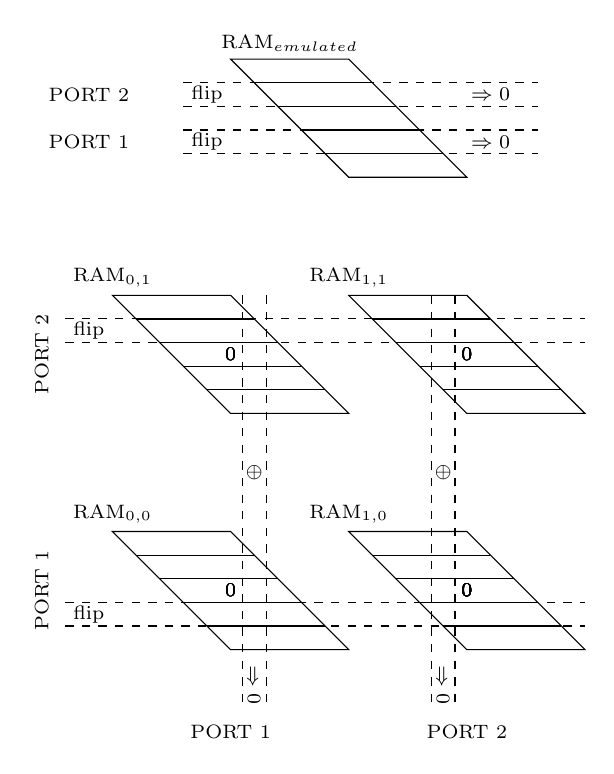
\begin{tikzpicture}[scale=3]
            \scriptsize
            \draw[] (.5,2-.25) -- (1,2-.25) -- (.5,2.25) -- (0, 2.25) -- cycle;
            \foreach \j in {-.15,-.05, .05, .15}{
                \draw[] (.25-\j, 2+\j) -- (.75-\j,2+\j);
            }
            \foreach \i/\v in {0/0,1/0,2/0,3/0,4/0}{
                \FPeval{\x}{.7-\i*.1};
                \FPeval{\y}{2-.2+\i*.1};
                \node[] at (\x,\y) {\v};
            }
            \node at (.25,2.25)[anchor=south]{RAM$_{emulated}$};
            \foreach \xram in {0,1}{
                \node at (\xram-.5,.25) [anchor=south]{RAM$_{\xram,0}$};
                \draw[xshift=\xram cm] (0,-.25) -- (.5,-.25) -- (0,.25) -- (-.5, .25) -- cycle;
                \foreach \j in {-.15,-.05, .05, .15}{
                    \draw[xshift=\xram cm] (-.25-\j, \j) -- (.25-\j,\j);
                }
                \def\y{0};
                \foreach \i/\v in {0/0,1/0,2/0,3/0,4/0}{
                    \FPeval{\x}{.2-\i*.1};
                    \FPeval{\y}{0-.2+\i*.1};
                    \node[] at (\x+\xram,\y) {\v};
                }
            }
            \foreach \xram in {0,1}{
                \node at (\xram-.5,1.25) [anchor=south]{RAM$_{\xram,1}$};
                \draw[xshift=\xram cm,yshift=1cm] (0,-.25) -- (.5,-.25) -- (0,.25) -- (-.5, .25) -- cycle;
                \foreach \j in {-.15,-.05, .05, .15}{
                    \draw[xshift=\xram cm,yshift=1cm] (-.25-\j, \j) -- (.25-\j,\j);
                }
                \def\y{0};
                \foreach \i/\v in {0/0,1/0,2/0,3/0,4/0}{
                    \FPeval{\x}{.2-\i*.1};
                    \FPeval{\y}{0-.2+\i*.1};
                    \node[] at (\x+\xram,\y+1) {\v};
                }
            }
            \node at (-.8,0)[rotate=90]{PORT 1};
            \node at (-.8,1)[rotate=90]{PORT 2};
            \node at (0,-.6){PORT 1};
            \node at (1,-.6){PORT 2};
            %TODO first and second
            \def\first{1};
            \ifthenelse{\first>0}{
            \draw[dashed] (-.7,0-.25+\first*.1) -- (1.5,0-.25+\first*.1);
            \draw[dashed] (-.7,0-.15+\first*.1) -- (1.5,0-.15+\first*.1);
            \draw[dashed] (0+.25-\first*.1,1.25) -- (0+.25-\first*.1,-.5);
            \draw[dashed] (0+.15-\first*.1,1.25) -- (0+.15-\first*.1,-.5);
            \node[rotate=270] at (0.2-\first*.1,-.4) {$\Rightarrow0$};
            \node at (0.2-\first*.1,.5) {$\oplus$};
            \node at (-.6,-.2+\first*.1) {flip};
        }{}
            \def\second{3};
            \ifthenelse{\second>0}{
            \draw[dashed] (-.7,1-.25+\second*.1) -- (1.5,1-.25+\second*.1);
            \draw[dashed] (-.7,1-.15+\second*.1) -- (1.5,1-.15+\second*.1);
            \draw[dashed] (1+.25-\second*.1,1.25) -- (1+.25-\second*.1,-.5);
            \draw[dashed] (1+.15-\second*.1,1.25) -- (1+.15-\second*.1,-.5);
            \node[rotate=270] at (1.2-\second*.1,-.4) {$\Rightarrow0$};
            \node at (1.2-\second*.1,.5) {$\oplus$};
            \node at (-.6,.8+\second*.1) {flip};
        }{}
            \ifthenelse{\first>0}{
            \draw[dashed] (-.2,2-.25+\first*.1) -- (1.3,2-.25+\first*.1);
            \draw[dashed] (-.2,2-.15+\first*.1) -- (1.3,2-.15+\first*.1);
            \node at (-.6,2-.2+\first*.1) {PORT 1};
            \node at (-.1,2-.2+\first*.1) {flip};
            \node at (1.1,2-.2+\first*.1) {$\Rightarrow0$};

        }{}
            \ifthenelse{\second>0}{
            \draw[dashed] (-.2,2-.25+\second*.1) -- (1.3,2-.25+\second*.1);
            \draw[dashed] (-.2,2-.15+\second*.1) -- (1.3,2-.15+\second*.1);
            \node at (-.6,2-.2+\second*.1) {PORT 2};
            \node at (-.1,2-.2+\second*.1) {flip};
            \node at (1.1,2-.2+\second*.1) {$\Rightarrow0$};
        }{}

        \end{tikzpicture}
        \caption{On the first clock cycle, Port 1 receives a request for cell 1 and Port 2 receives a request for cell 3.}
        \label{fig:xorram0}
    \end{subfigure}
    \begin{subfigure}{.5\linewidth}
        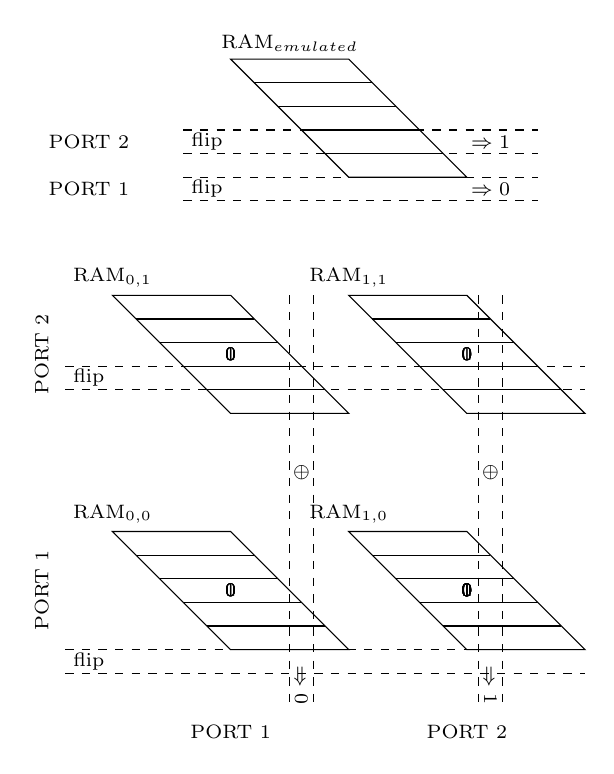
\begin{tikzpicture}[scale=3]
            \scriptsize
            \draw[] (.5,2-.25) -- (1,2-.25) -- (.5,2.25) -- (0, 2.25) -- cycle;
            \foreach \j in {-.15,-.05, .05, .15}{
                \draw[] (.25-\j, 2+\j) -- (.75-\j,2+\j);
            }
            \foreach \i/\v in {0/0,1/1,2/0,3/1,4/0}{
                \FPeval{\x}{.7-\i*.1};
                \FPeval{\y}{2-.2+\i*.1};
                \node[] at (\x,\y) {\v};
            }
            \node at (.25,2.25)[anchor=south]{RAM$_{emulated}$};
            \foreach \xram in {0,1}{
                \node at (\xram-.5,.25) [anchor=south]{RAM$_{\xram,0}$};
                \draw[xshift=\xram cm] (0,-.25) -- (.5,-.25) -- (0,.25) -- (-.5, .25) -- cycle;
                \foreach \j in {-.15,-.05, .05, .15}{
                    \draw[xshift=\xram cm] (-.25-\j, \j) -- (.25-\j,\j);
                }
                \def\y{0};
                \foreach \i/\v in {0/0,1/1,2/0,3/0,4/0}{
                    \FPeval{\x}{.2-\i*.1};
                    \FPeval{\y}{0-.2+\i*.1};
                    \node[] at (\x+\xram,\y) {\v};
                }
            }
            \foreach \xram in {0,1}{
                \node at (\xram-.5,1.25) [anchor=south]{RAM$_{\xram,1}$};
                \draw[xshift=\xram cm,yshift=1cm] (0,-.25) -- (.5,-.25) -- (0,.25) -- (-.5, .25) -- cycle;
                \foreach \j in {-.15,-.05, .05, .15}{
                    \draw[xshift=\xram cm,yshift=1cm] (-.25-\j, \j) -- (.25-\j,\j);
                }
                \def\y{0};
                \foreach \i/\v in {0/0,1/0,2/0,3/1,4/0}{
                    \FPeval{\x}{.2-\i*.1};
                    \FPeval{\y}{0-.2+\i*.1};
                    \node[] at (\x+\xram,\y+1) {\v};
                }
            }
            \node at (-.8,0)[rotate=90]{PORT 1};
            \node at (-.8,1)[rotate=90]{PORT 2};
            \node at (0,-.6){PORT 1};
            \node at (1,-.6){PORT 2};
            %TODO first and second
            \def\first{-1};
            \ifthenelse{\first>0}{
            \draw[dashed] (-.7,0-.25+\first*.1) -- (1.5,0-.25+\first*.1);
            \draw[dashed] (-.7,0-.15+\first*.1) -- (1.5,0-.15+\first*.1);
            \draw[dashed] (0+.25-\first*.1,1.25) -- (0+.25-\first*.1,-.5);
            \draw[dashed] (0+.15-\first*.1,1.25) -- (0+.15-\first*.1,-.5);
            \node[rotate=270] at (0.2-\first*.1,-.4) {$\Rightarrow 0$};
            \node at (0.2-\first*.1,.5) {$\oplus$};
            \node at (-.6,-.2+\first*.1) {flip};
        }{}
            \def\second{1};
            \ifthenelse{\second>0}{
            \draw[dashed] (-.7,1-.25+\second*.1) -- (1.5,1-.25+\second*.1);
            \draw[dashed] (-.7,1-.15+\second*.1) -- (1.5,1-.15+\second*.1);
            \draw[dashed] (1+.25-\second*.1,1.25) -- (1+.25-\second*.1,-.5);
            \draw[dashed] (1+.15-\second*.1,1.25) -- (1+.15-\second*.1,-.5);
            \node[rotate=270] at (1.2-\second*.1,-.4) {$\Rightarrow 1$};
            \node at (1.2-\second*.1,.5) {$\oplus$};
            \node at (-.6,.8+\second*.1) {flip};
        }{}
            \ifthenelse{\first>0}{
            \draw[dashed] (-.2,2-.25+\first*.1) -- (1.3,2-.25+\first*.1);
            \draw[dashed] (-.2,2-.15+\first*.1) -- (1.3,2-.15+\first*.1);
            \node at (-.6,2-.2+\first*.1) {PORT 1};
            \node at (-.1,2-.2+\first*.1) {flip};
            \node at (1.1,2-.2+\first*.1) {$\Rightarrow 0$};

        }{}
            \ifthenelse{\second>0}{
            \draw[dashed] (-.2,2-.25+\second*.1) -- (1.3,2-.25+\second*.1);
            \draw[dashed] (-.2,2-.15+\second*.1) -- (1.3,2-.15+\second*.1);
            \node at (-.6,2-.2+\second*.1) {PORT 2};
            \node at (-.1,2-.2+\second*.1) {flip};
            \node at (1.1,2-.2+\second*.1) {$\Rightarrow 1$};
        }{}

        \end{tikzpicture}
        \caption{On the second clock cycle, Port 2 receives a request for cell 1 and Port 1 does not receive a request.}
        \label{fig:xorram1}
    \end{subfigure}
    \begin{subfigure}{.5\linewidth}
        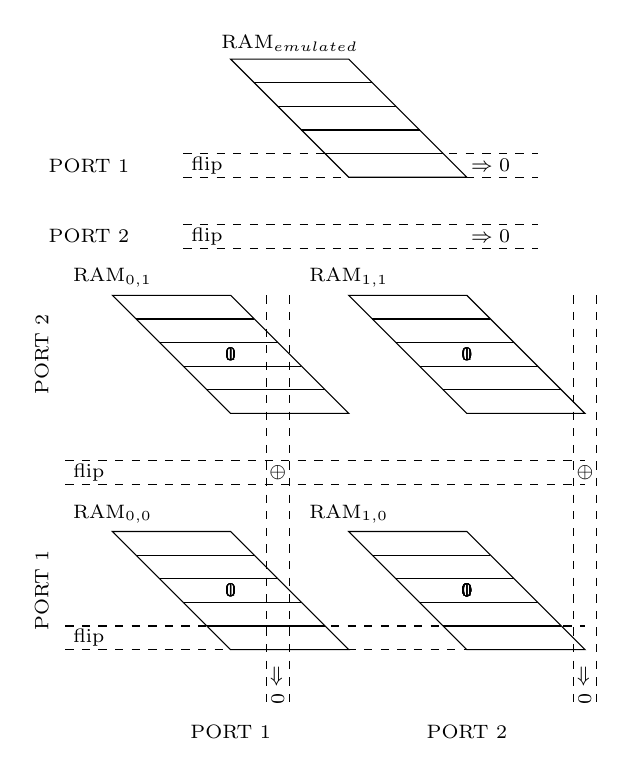
\begin{tikzpicture}[scale=3]
            \scriptsize
            \draw[] (.5,2-.25) -- (1,2-.25) -- (.5,2.25) -- (0, 2.25) -- cycle;
            \foreach \j in {-.15,-.05, .05, .15}{
                \draw[] (.25-\j, 2+\j) -- (.75-\j,2+\j);
            }
            \foreach \i/\v in {0/0,1/0,2/0,3/1,4/0}{
                \FPeval{\x}{.7-\i*.1};
                \FPeval{\y}{2-.2+\i*.1};
                \node[] at (\x,\y) {\v};
            }
            \node at (.25,2.25)[anchor=south]{RAM$_{emulated}$};
            \foreach \xram in {0,1}{
                \node at (\xram-.5,.25) [anchor=south]{RAM$_{\xram,0}$};
                \draw[xshift=\xram cm] (0,-.25) -- (.5,-.25) -- (0,.25) -- (-.5, .25) -- cycle;
                \foreach \j in {-.15,-.05, .05, .15}{
                    \draw[xshift=\xram cm] (-.25-\j, \j) -- (.25-\j,\j);
                }
                \def\y{0};
                \foreach \i/\v in {0/0,1/1,2/0,3/0,4/0}{
                    \FPeval{\x}{.2-\i*.1};
                    \FPeval{\y}{0-.2+\i*.1};
                    \node[] at (\x+\xram,\y) {\v};
                }
            }
            \foreach \xram in {0,1}{
                \node at (\xram-.5,1.25) [anchor=south]{RAM$_{\xram,1}$};
                \draw[xshift=\xram cm,yshift=1cm] (0,-.25) -- (.5,-.25) -- (0,.25) -- (-.5, .25) -- cycle;
                \foreach \j in {-.15,-.05, .05, .15}{
                    \draw[xshift=\xram cm,yshift=1cm] (-.25-\j, \j) -- (.25-\j,\j);
                }
                \def\y{0};
                \foreach \i/\v in {0/0,1/1,2/0,3/1,4/0}{
                    \FPeval{\x}{.2-\i*.1};
                    \FPeval{\y}{0-.2+\i*.1};
                    \node[] at (\x+\xram,\y+1) {\v};
                }
            }
            \node at (-.8,0)[rotate=90]{PORT 1};
            \node at (-.8,1)[rotate=90]{PORT 2};
            \node at (0,-.6){PORT 1};
            \node at (1,-.6){PORT 2};
            %TODO first and second
            \def\first{0};
            \ifthenelse{\first>-1}{
            \draw[dashed] (-.7,0-.25+\first*.1) -- (1.5,0-.25+\first*.1);
            \draw[dashed] (-.7,0-.15+\first*.1) -- (1.5,0-.15+\first*.1);
            \draw[dashed] (0+.25-\first*.1,1.25) -- (0+.25-\first*.1,-.5);
            \draw[dashed] (0+.15-\first*.1,1.25) -- (0+.15-\first*.1,-.5);
            \node[rotate=270] at (0.2-\first*.1,-.4) {$\Rightarrow 0$};
            \node at (0.2-\first*.1,.5) {$\oplus$};
            \node at (-.6,-.2+\first*.1) {flip};
        }{}
            \def\second{-3};
            \ifthenelse{\second>0}{
            \draw[dashed] (-.7,1-.25+\second*.1) -- (1.5,1-.25+\second*.1);
            \draw[dashed] (-.7,1-.15+\second*.1) -- (1.5,1-.15+\second*.1);
            \draw[dashed] (1+.25-\second*.1,1.25) -- (1+.25-\second*.1,-.5);
            \draw[dashed] (1+.15-\second*.1,1.25) -- (1+.15-\second*.1,-.5);
            \node[rotate=270] at (1.2-\second*.1,-.4) {$\Rightarrow 0$};
            \node at (1.2-\second*.1,.5) {$\oplus$};
            \node at (-.6,.8+\second*.1) {flip};
        }{}
            \ifthenelse{\first>-1}{
            \draw[dashed] (-.2,2-.25+\first*.1) -- (1.3,2-.25+\first*.1);
            \draw[dashed] (-.2,2-.15+\first*.1) -- (1.3,2-.15+\first*.1);
            \node at (-.6,2-.2+\first*.1) {PORT 1};
            \node at (-.1,2-.2+\first*.1) {flip};
            \node at (1.1,2-.2+\first*.1) {$\Rightarrow 0$};

        }{}
            \ifthenelse{\second>0}{
            \draw[dashed] (-.2,2-.25+\second*.1) -- (1.3,2-.25+\second*.1);
            \draw[dashed] (-.2,2-.15+\second*.1) -- (1.3,2-.15+\second*.1);
            \node at (-.6,2-.2+\second*.1) {PORT 2};
            \node at (-.1,2-.2+\second*.1) {flip};
            \node at (1.1,2-.2+\second*.1) {$\Rightarrow 0$};
        }{}

        \end{tikzpicture}
        \caption{On the third clock cycle, Port 1 receives a request for cell 0 and Port 2 does not receive a request.}
        \label{fig:xorram2}
    \end{subfigure}
    \begin{subfigure}{.5\linewidth}
        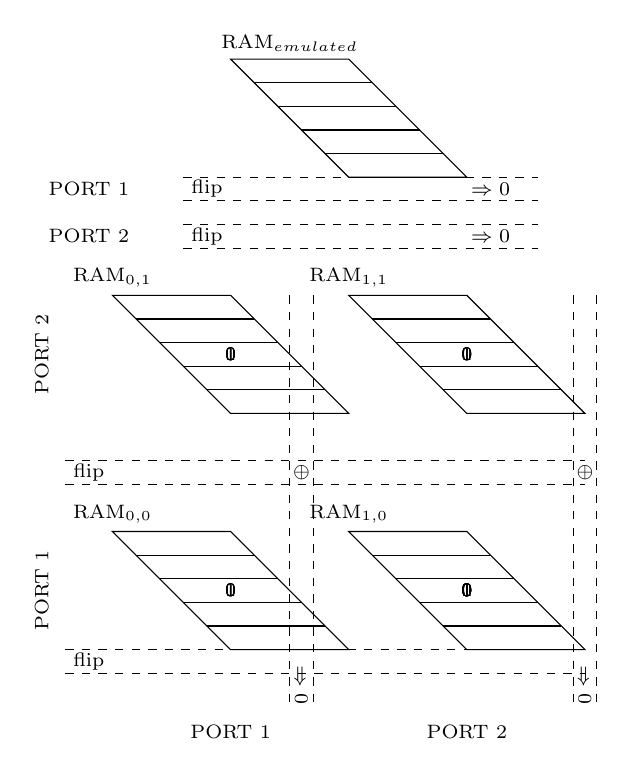
\begin{tikzpicture}[scale=3]
            \scriptsize
            \draw[] (.5,2-.25) -- (1,2-.25) -- (.5,2.25) -- (0, 2.25) -- cycle;
            \foreach \j in {-.15,-.05, .05, .15}{
                \draw[] (.25-\j, 2+\j) -- (.75-\j,2+\j);
            }
            \foreach \i/\v in {0/1,1/0,2/0,3/1,4/0}{
                \FPeval{\x}{.7-\i*.1};
                \FPeval{\y}{2-.2+\i*.1};
                \node[] at (\x,\y) {\v};
            }
            \node at (.25,2.25)[anchor=south]{RAM$_{emulated}$};
            \foreach \xram in {0,1}{
                \node at (\xram-.5,.25) [anchor=south]{RAM$_{\xram,0}$};
                \draw[xshift=\xram cm] (0,-.25) -- (.5,-.25) -- (0,.25) -- (-.5, .25) -- cycle;
                \foreach \j in {-.15,-.05, .05, .15}{
                    \draw[xshift=\xram cm] (-.25-\j, \j) -- (.25-\j,\j);
                }
                \def\y{0};
                \foreach \i/\v in {0/1,1/1,2/0,3/0,4/0}{
                    \FPeval{\x}{.2-\i*.1};
                    \FPeval{\y}{0-.2+\i*.1};
                    \node[] at (\x+\xram,\y) {\v};
                }
            }
            \foreach \xram in {0,1}{
                \node at (\xram-.5,1.25) [anchor=south]{RAM$_{\xram,1}$};
                \draw[xshift=\xram cm,yshift=1cm] (0,-.25) -- (.5,-.25) -- (0,.25) -- (-.5, .25) -- cycle;
                \foreach \j in {-.15,-.05, .05, .15}{
                    \draw[xshift=\xram cm,yshift=1cm] (-.25-\j, \j) -- (.25-\j,\j);
                }
                \def\y{0};
                \foreach \i/\v in {0/0,1/1,2/0,3/1,4/0}{
                    \FPeval{\x}{.2-\i*.1};
                    \FPeval{\y}{0-.2+\i*.1};
                    \node[] at (\x+\xram,\y+1) {\v};
                }
            }
            \node at (-.8,0)[rotate=90]{PORT 1};
            \node at (-.8,1)[rotate=90]{PORT 2};
            \node at (0,-.6){PORT 1};
            \node at (1,-.6){PORT 2};
            %TODO first and second
            \def\first{-1};
            \ifthenelse{\first>0}{
            \draw[dashed] (-.7,0-.25+\first*.1) -- (1.5,0-.25+\first*.1);
            \draw[dashed] (-.7,0-.15+\first*.1) -- (1.5,0-.15+\first*.1);
            \draw[dashed] (0+.25-\first*.1,1.25) -- (0+.25-\first*.1,-.5);
            \draw[dashed] (0+.15-\first*.1,1.25) -- (0+.15-\first*.1,-.5);
            \node[rotate=270] at (0.2-\first*.1,-.4) {$\Rightarrow 0$};
            \node at (0.2-\first*.1,.5) {$\oplus$};
            \node at (-.6,-.2+\first*.1) {flip};
        }{}
            \def\second{-3};
            \ifthenelse{\second>0}{
            \draw[dashed] (-.7,1-.25+\second*.1) -- (1.5,1-.25+\second*.1);
            \draw[dashed] (-.7,1-.15+\second*.1) -- (1.5,1-.15+\second*.1);
            \draw[dashed] (1+.25-\second*.1,1.25) -- (1+.25-\second*.1,-.5);
            \draw[dashed] (1+.15-\second*.1,1.25) -- (1+.15-\second*.1,-.5);
            \node[rotate=270] at (1.2-\second*.1,-.4) {$\Rightarrow 0$};
            \node at (1.2-\second*.1,.5) {$\oplus$};
            \node at (-.6,.8+\second*.1) {flip};
        }{}
            \ifthenelse{\first>0}{
            \draw[dashed] (-.2,2-.25+\first*.1) -- (1.3,2-.25+\first*.1);
            \draw[dashed] (-.2,2-.15+\first*.1) -- (1.3,2-.15+\first*.1);
            \node at (-.6,2-.2+\first*.1) {PORT 1};
            \node at (-.1,2-.2+\first*.1) {flip};
            \node at (1.1,2-.2+\first*.1) {$\Rightarrow 0$};

        }{}
            \ifthenelse{\second>0}{
            \draw[dashed] (-.2,2-.25+\second*.1) -- (1.3,2-.25+\second*.1);
            \draw[dashed] (-.2,2-.15+\second*.1) -- (1.3,2-.15+\second*.1);
            \node at (-.6,2-.2+\second*.1) {PORT 2};
            \node at (-.1,2-.2+\second*.1) {flip};
            \node at (1.1,2-.2+\second*.1) {$\Rightarrow 0$};
        }{}

        \end{tikzpicture}
        \caption{On the fourth clock cycle, neither Port 1 or Port 2 receives a request.}
        \label{fig:xorram3}
    \end{subfigure}
    \caption[Dual port RAM with zero clock cycle read latency]{This example shows 4 clock cycles of operation of a $1\times 5$ dual port RAM, created by combining 4 pseudo dual-port RAMs.}
    \label{fig:xorram}
\end{figure}
%TODO: synthesis results
\section{Results}
The two important metrics for most MACs are the throughput and synthesis results.
\subsection{Throughput}
Although the MAC rarely stalls in theory. We thought it would be important to show this in practice as well. We use the matricies from the benchmark and show the percent of time the MAC stalls in each case. We should this in figure X.
\subsection{Synthesis}
We placed and routed one MAC using xst (Xilinx Synthesis Tools). The frequency of the MAC was 423Mhz. The MAC used 3,105 Registers, 3,236 LUTs, 5.5 RAM blocks, and 7 DSP (multiplier) blocks. By default xst uses RAM blocks for the FIFO even though their depth is equal to 32. XST can be forced to use LUTs, which would use 112 more LUTs and 3.5 fewer RAM blocks.
